\section{Distributed Web Crawler}\label{sec:distributed_web_crawler}

The performance of the distributed web crawler is dependent on three main factors:
\begin{itemize}
    \item The number of URLs each crawler instance is assigned to crawl.
    \item The rate at which new crawler instances are spawned.
    \item The error rate of the crawling process.
\end{itemize}

During the testing phase, the following settings were used to evaluate the performance of the distributed web crawler:
\begin{itemize}
    \item Each crawler instance was assigned to crawl 100 URLs.
    \item The rate at which new crawler instances were spawned was set to 1 instance every 3 minutes (20 instances per hour) - across 3 AWS regions.
\end{itemize}

During a period of 24 hours, the distributed web crawler was able to successfully crawl a total of 29,809 unique URLs from a collection of 36 websites, which represents an average of 1,242 URLs crawled per hour.
Table~\ref{tab:crawler_last_updated_24h} shows the total number of pages crawled per domain, as well as the number of pages that were updated within the last 24 hours.

\begin{table}[H]
    \centering
    \begin{tabular}{lrr}
        \toprule
        \textbf{Domain} & \textbf{Total Pages} & \textbf{Updated in 24h} \\
        \midrule
        abansit.lk & 286 & 129 \\
        barclays.lk & 2876 & 841 \\
        bigdeals.lk & 53606 & 9884 \\
        brownsdeals.com & 795 & 184 \\
        buyabans.com & 10363 & 3509 \\
        buyzone.lk & 308 & 75 \\
        celltronics.lk & 2508 & 998 \\
        chamacomputers.lk & 3360 & 1450 \\
        damro.lk & 1662 & 549 \\
        dialcom.lk & 577 & 174 \\
        finez.lk & 409 & 118 \\
        fireworks.lk & 1608 & 594 \\
        gamestreet.lk & 2640 & 1206 \\
        geniusmobile.lk & 680 & 270 \\
        homelux.lk & 239 & 57 \\
        idealz.lk & 236 & 39 \\
        laptop.lk & 2000 & 715 \\
        lifemobile.lk & 3497 & 0 \\
        luxuryx.lk & 1266 & 185 \\
        mansafit.com & 713 & 93 \\
        mcentre.lk & 721 & 294 \\
        mysoftlogic.lk & 762 & 174 \\
        nanotek.lk & 2219 & 674 \\
        onei.lk & 5161 & 1962 \\
        pettahkade.lk & 545 & 154 \\
        raesl.lk & 315 & 49 \\
        redlinetech.lk & 3154 & 380 \\
        rooter.lk & 293 & 150 \\
        simplytek.lk & 3127 & 1383 \\
        singersl.com & 4328 & 1357 \\
        singhagiri.lk & 817 & 199 \\
        strong.lk & 349 & 91 \\
        techzone.lk & 1998 & 964 \\
        ugreen.lk & 1251 & 330 \\
        xclusive.lk & 1198 & 242 \\
        xmobile.lk & 1095 & 336 \\
        \midrule
        \textbf{TOTAL} & \textbf{116,962} & \textbf{29,809} \\
        \bottomrule
    \end{tabular}
    \caption{Per-domain crawl totals and URL updates within the last 24 hours.}
    \label{tab:crawler_last_updated_24h}
\end{table}

During this same period, there were a total of \texttt{972} errors encountered by the distributed web crawler, which represents an error rate of approximately 3.26\% of the total URLs crawled.
However, many of these URLs were crawled successfully on retry.
Of which,
\begin{itemize}
    \item \texttt{324} were timeout errors, which represents instances where the crawler was unable to establish a connection to the target website and render the webpage within the specified timeout period.
    \item \texttt{458} were HTTP 403 errors, which indicates that the crawler was denied access to the target website by the website's server.
    \item \texttt{42} were HTTP 404 errors, which indicates that the requested URL was not found on the target website.
    \item \texttt{30} were HTTP 429 errors, which indicates that the crawler was rate-limited by the target website due to too many requests being sent in a short period of time.
\end{itemize}

Out of the total of 116,962 unique URLs crawled, \texttt{73,354} were classified as product pages, while \texttt{44,063} were classified as non-product pages.
If only the product pages are considered, within the last 3 days, a total of \texttt{71,696} URLs were crawled, which means that \texttt{1,658} pages missed the 72-hour update requirement.
Of these, \texttt{1,651} were from a single domain (\texttt{lifemobile.lk}), which seems to have implemented aggressive anti-bot measures, preventing the crawler from accessing and crawling the product pages on their website.

Figure~\ref{fig:crawler_velocity} shows the velocity of the distributed web crawler over a period of 30 days, which represents the number of unique URLs in 30-minute intervals that were successfully crawled and stored in the database along with a moving average of the velocity over a 24-hour period.
It also shows the effect of the anti-bot measures implemented by CloudFlare, and the steps taken to mitigate the impact of these measures on the crawling process, which includes reducing the crawling rate and implementing anti-bot measures.

\begin{figure}[H]
    \centering
    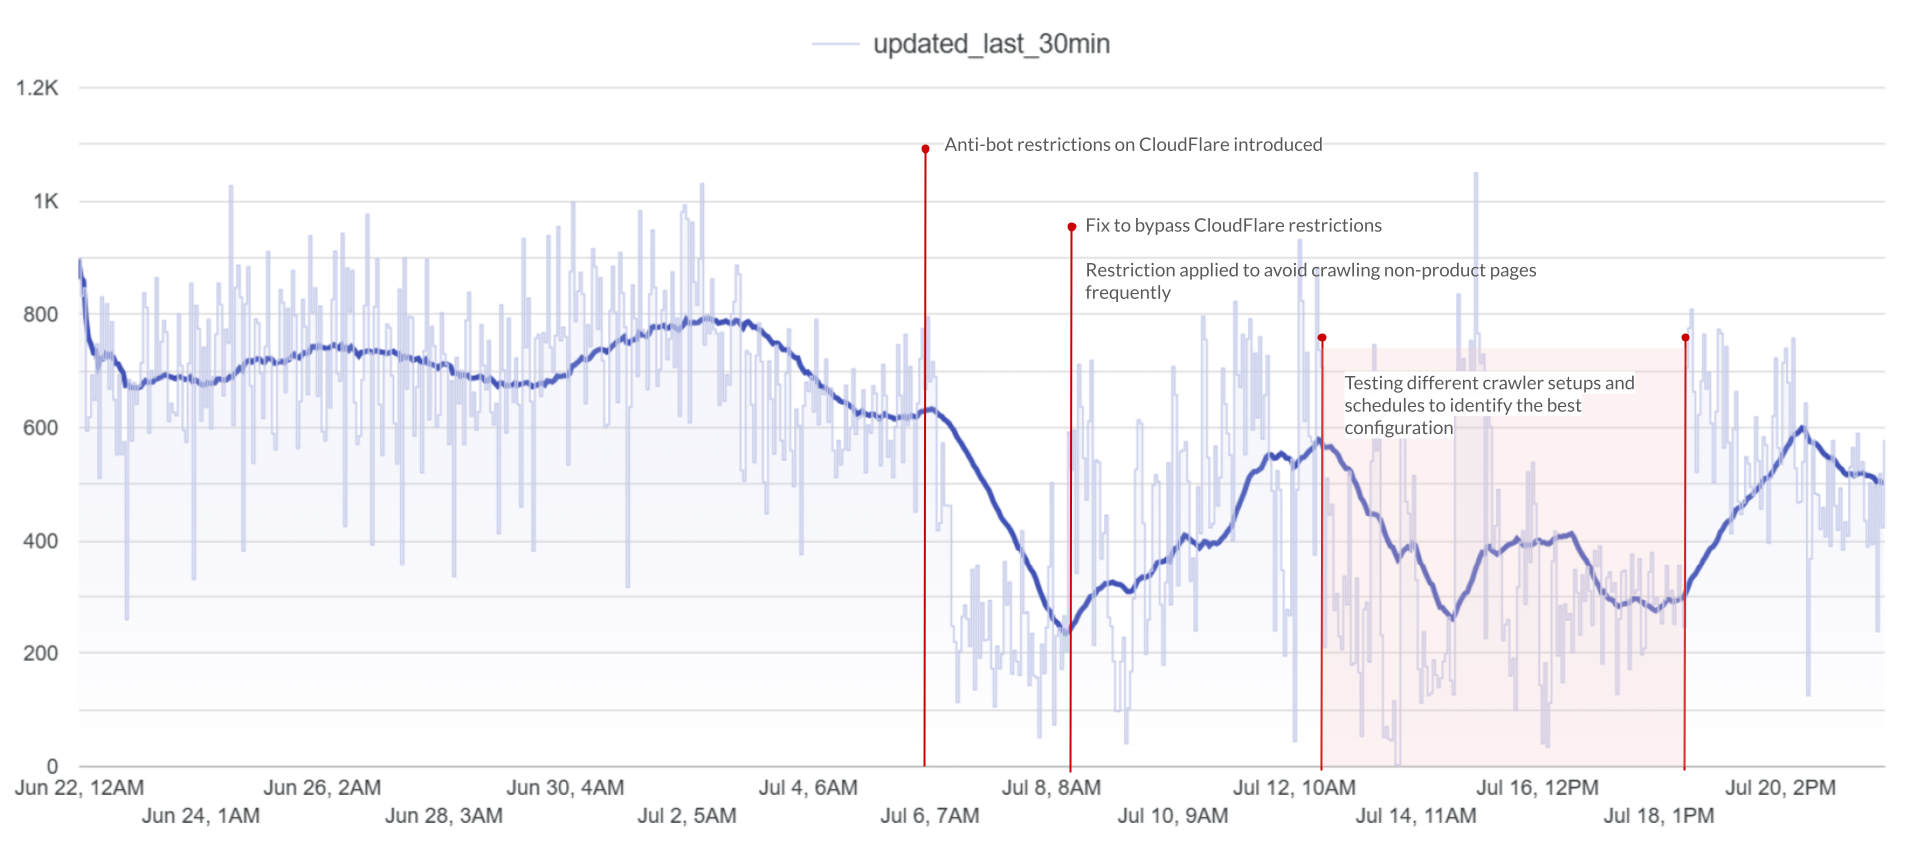
\includegraphics[width=1\textwidth]{images/crawler_velocity}
    \caption{Distributed crawler velocity over 30 days}
    \label{fig:crawler_velocity}
\end{figure}